\section{Granica ciągu}
% a_{n} A(n)

\subsection{Definicja}

\subsubsection{Definicja matematyczna}

\noindent
\textbf{Wersja ogólna}
\newline
Dla dowolnej przestrzeni o~dowolnej metryce (mierze odległości).
\newline
$$\exists_{g \in X} \lim_{n \to \infty} A(n) = g \iff \forall_{\varepsilon>0} \exists_{N \in \N} \forall_{n \geq N}  \rho(A(n), g) < \varepsilon$$
słownie: Ciąg $(A(n))$ dąży do~$g$ z~przestrzeni~$X$ przy~$g$ dążącym do~nieskończoności wtedy i~tylko wtedy, gdy dla~dowolnego dodatniego~$\varepsilon$ (czyt.~„epsilon”) istnieje liczba~$N$ takie, że~dla dowolnego~$n$ większego od~$N$ odległość ($\rho$, czyt.~„ro”) pomiędzy n-tym wyrazem ciągu~$A$ a~liczbą~$g$ jest mniejsza niż~$\varepsilon$.
\newline

\noindent
\textbf{Wersja nam przydatna}
\newline
Czyli w~metryce euklidesowej dla~przestrzeni jednowymiarowej, tzn.~na~prostej z~liczbami rzeczywistymi, gdzie odległość między punktami liczymy wartością bezwzględną, czyli $\rho(x, y) = \left|x - y\right|$
\newline
$$\exists_{g \in \R} \lim_{n \to \infty} A(n) = g \iff \forall_{\varepsilon>0} \exists_{N \in \N} \forall_{n \geq N} \left|A(n) - g\right| < \varepsilon $$
słownie: Ciąg $(A(n))$ dąży do~liczby rzeczywistej~$g$ przy $n$~dążącym do~nieskończoności wtedy i~tylko wtedy, gdy dla~dowolnego dodatniego~$\varepsilon$ (czyt.~„epsilon”) istnieje liczba $N$ taka, że~dla dowolnej liczby~$n$ większej od~$N$ różnica bezwzględna pomiędzy n-tym wyrazem ciągu~$A$ a~liczbą~$g$ jest mniejsza niż~$\varepsilon$.
\newline

\noindent
\textbf{Inne nazewnictwa}
\begin{itemize}
    \item $\lim_{n \to \infty} A(n) = g$ możemy też zapisać w postaci \newline $A(n) \to g$ $(n \to \infty)$.
    \item Zamiast czytać „ciąg~$(A(n))$ dąży do~$g$ przy~$n$ dążącym do~nieskończoności” można również czytać „ciąg~$(A(n))$ jest zbieżny do~$g$ przy~$n$ dążącym do~nieskończoności” lub „granica ciągu~$(A(n))$ przy~$n$ dążącym do~nieskończoności wynosi~$g$”.
\end{itemize}
\indent

\subsubsection{Na chłopski rozum}
Mamy ciąg z~elementami ponumerowanymi indeksami 0, 1, 2, 3... (czyli $A(0)$, $A(1)$, $A(2)$, $A(3)$, ...). Ciąg taki dąży wartościami do~pewnej liczby~$g$, 
jeżeli –~ustaliwszy pewną dowolną małą liczbę (epsilon, $\varepsilon$) –~znajdziemy taką liczbę~$N$, że~zarówno odległość między~$A(N)$ a liczbą~$g$ jest mniejsza od~naszej małej liczby~$\varepsilon$, 
jak~i każdy następny wyraz jest odległy od~g o~mniej niż $\varepsilon$. Wówczas prawie wszystkie wyrazy ciągu (wszystkie poza skończoną liczbą, tj.~od~$0$ do~$N-1$) znajdują się w~przedziale wartości $(g-\varepsilon, g+\varepsilon)$. 
Z~dowolności ustalenia epsilona wynika, że~w~nieskończoności te liczby dążą do~$g$, jak widać na~poniższym przykładzie.
\begin{figure}[H]
    \caption{Wykres ciagu $A(n) = (-1)^n * \frac{1}{n}$}
    \centering
        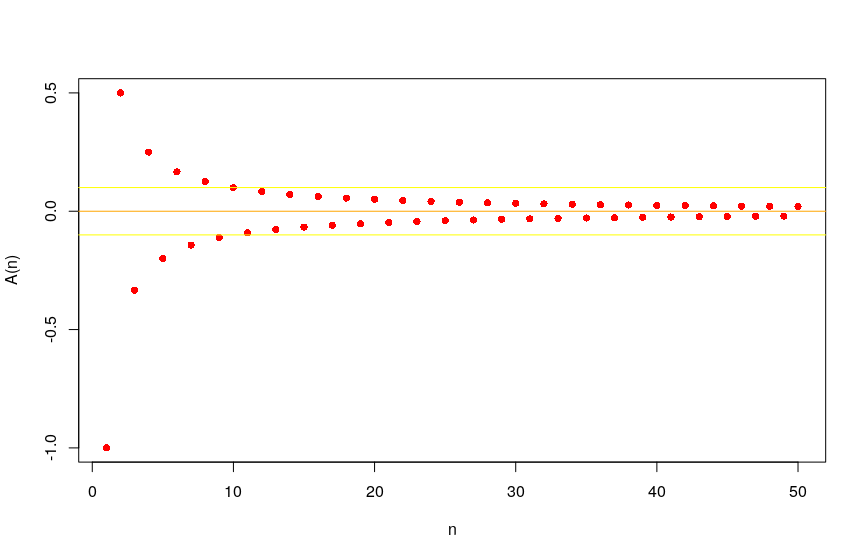
\includegraphics[width=0.75\textwidth]{photos/granica1.png}
\end{figure}
Widzimy, po~ustaleniu pewnej liczby $\varepsilon$, że~prawie wszystkie wartości ciągu znajdują~się w~obrębie przedziału $(g-\varepsilon, g+\varepsilon)$ (zaznaczone jest to żółtymi prostymi), a~w~nieskończoności zbliżają~się do~liczby~$g$ (zaznaczona pomarańczową prostą). 
Zatem ciąg~$(A(n))$ zbiega do~liczby~$g$.
W powyższym przypadku możemy zapisać to tak:
\begin{itemize}
    \item $A(n) = (-1)^n * \frac{1}{n} \to 0$ $(n \to \infty)$,
    \item $\lim_{n \to \infty} A(n) = (-1)^n * \frac{1}{n} = 0$.
\end{itemize} 

\newpage
\subsection{Własności}

\textbf{Uwaga:} Rozpatrujemy tutaj granice ciągów na~prostej rzeczywistej z~wartością bezwzględną jako~miarą odległości (mianowicie $\rho(x, y) = \left|x - y\right|$).

\begin{fakt}
Ciąg ma co~najwyżej jedną granicę (właściwą) –~mianowicie może mieć jedną granicę, lub~nie~mieć jej wcale.
\end{fakt}

\begin{tw}
    Jeśli ciąg ma~granicę właściwą, to~jest on~ograniczony.
\end{tw}
\begin{dow}
    \begin{enumerate}
        \item Niech dany będzie ciąg $(A(n))$ zbieżny do~$g$. Niech $\varepsilon=1$. 
        \item Wtedy z~definicji zbieżności istnieje takie $N$, że~dla każdego $n>N$ zachodzi $|A(n)-g| < 1$.
        \item Z~własności wartości bezwzględnej otrzymujemy: $$ -1-|g|\leqslant -1+g<A(n)<1+g \leqslant 1+|g|, $$ co~oznacza że~$|A(n)|<1+|g|$.
        \item Weźmy $M=\max\{|A(1)|, |A(2)|, \dots, |A(N)|, 1+|g|\}$. Zbiór jest skończony, a zatem istnieje jedno wspólne ograniczenie wszystkich elementów ciagu A(n), co oznacza, że jest ograniczony.~\cite{granice1}
    \end{enumerate}
\end{dow}

\begin{fakt}
    Dowolny nieskończony podciąg ciągu zbieżnego jest zbieżny do tej samej granicy.
\end{fakt}

\begin{fakt}
    Jeśli ciągi $(A(n))$ i $(B(n))$ są zbieżne oraz $ A(n) \leqslant B(n)$ dla każdego naturalnego $n$, to $lim_{n \to \infty} A(n) \leqslant lim_{n \to \infty} B(n)$.
\end{fakt}

\begin{tw}
    \label{bolwei}
		(o trzech ciągach)
    Jeśli ciągi $A(n)$ i~$C(n)$ są zbieżne do~wspólnej granicy $g$, przy czym $ A(n) \leqslant B(n) \leqslant C(n) $ dla każdego naturalnego $n$, to~ciąg $B(n)$ również jest zbieżny 
    i~to do~granicy $g$.
\end{tw}
\begin{dow}
    \begin{enumerate}
        \item Ustalmy $\varepsilon > 0$. 
        \item Ciąg $(A(n))$ jest zbieżny do~$g$, zatem istnieje liczba $N_1$ taka, że~dla każdego $n>N_1$ zachodzi $|A(n)-g| < \varepsilon$.
        \item Ciąg $(C(n))$ jest zbieżny do~$g$, zatem istnieje liczba $N_2$ taka, że~dla każdego $n>N_2$ zachodzi $|C(n)-g| < \varepsilon$.
        \item Weźmy $N = \max(N_1, N_2)$. Wówczas dla dowolnego $n>N$ zachodzą nierówności: $|A(n)-g| < \varepsilon$ oraz $|C(n)-g| <  \varepsilon$.~\cite{granice2}
        \item Stąd, z~własności wartości bezwzględnej, mamy nierówności\newline $-\varepsilon < A(n)-g$ oraz $C(n)-g < \varepsilon$,\newline czyli $g-\varepsilon < A(n)$ oraz $C(n) < g+\varepsilon$.
        \item Zatem, korzystając z~założenia o~nierównościach wyrazów ciągów $(A(n))$, $(B(n))$, $(C(n))$, zachodzi $$g-\varepsilon < A(n) \leqslant B(n) \leqslant C(n) < g+\varepsilon,$$ 
        czyli $|B(n) - g| < \varepsilon$.
        \item Z powyższego wynika, że~$\lim_{n \to \infty} B(n) = g$.~\cite{granice2}
    \end{enumerate}
\end{dow}

\newpage
\subsection{Przykłady}

\begin{enumerate}
    \item Weźmy $\lim_{n \to \infty} \sqrt[n]{2^n + 3^n + 4^n}$. Wiemy, że dla każdego naturalnego $n$ zachodzi 
    $$ \sqrt[n]{4^n} \leqslant \sqrt[n]{2^n + 3^n + 4^n} \leqslant \sqrt[n]{4^n + 4^n + 4^n} $$
    $$ \sqrt[n]{4^n} \leqslant \sqrt[n]{2^n + 3^n + 4^n} \leqslant \sqrt[n]{3 * 4^n} $$
    Wiemy, że $\lim_{n \to \infty} \sqrt[n]{4^n} = 4$ oraz $\lim_{n \to \infty} \sqrt[n]{3*4^n} = 4$. 
    Zatem, korzystając z twierdzenia o trzech ciągach,
    $$ \lim_{n \to \infty} \sqrt[n]{4^n} \leqslant \lim_{n \to \infty} \sqrt[n]{2^n + 3^n + 4^n} \leqslant \lim_{n \to \infty} \sqrt[n]{3 * 4^n} $$
    $$ 4 \leqslant \lim_{n \to \infty} \sqrt[n]{2^n + 3^n + 4^n} \leqslant 4 $$
    Stąd, $\lim_{n \to \infty} \sqrt[n]{2^n + 3^n + 4^n} = 4$.
\end{enumerate}

\newpage
\subsection{Zadania}